\chapter{$\zg$+Jets at the LHC}
\label{chap:Zs}

	\section{$Z$+jets}
	\label{sec:Zcurrents}

		Similarly to the the case of $W^\pm$ plus jets there are \emph{four} possible emission sites for the boson; Two on the forward incoming quark, and two on the backward incoming quarks (see figure \ref{fig:emissionsites}).

		\begin{figure}[h]
		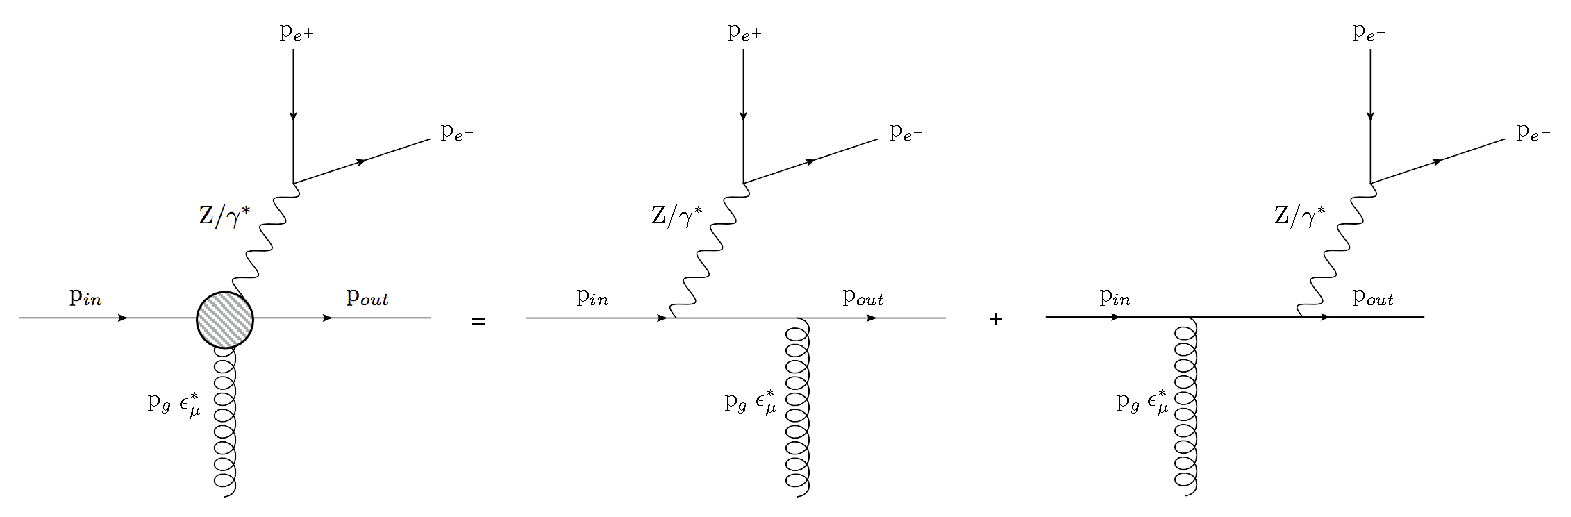
\includegraphics[width=0.98\linewidth]{figures/EmissionSites.pdf}
		\caption{The possible emission sites for a neutral weak boson.}
		\label{fig:emissionsites}
		\end{figure}

		In the language of currents (see for \emph{e.g.} \cite{Constructing}) we call the left hand side of figure \ref{fig:emissionsites} $j_\mu^\zg$:

		\begin{equation}
		j_\mu^Z = \overline{u}^{h_{out}}(p_{out})\left(\gamma^\sigma\frac{\slashed p_{out} + \slashed p_Z}{(p_{out} + p_Z)^2}\gamma_\mu + \gamma_\mu\frac{\slashed p_{in} - \slashed p_Z}{(p_{in} - p_Z)^2}\gamma_\sigma\right)u^{h_{in}}(p_{in})\times\overline{u}^{h_{e^-}}(p_{e^-})\gamma_\sigma u^{h_{e^+}}(p_{e^+}).
		\end{equation}

		We can then express amplitudes in terms of contractions of `emitting' and `non-emitting' currents.\\As the figure above indicates, when emitting a $Z$ boson there is also the possiblity of an off-shell photon being exchanged instead of a $Z$.  Since the difference in these two channels is indistinguishable 	in the final state we must treat the interference as the amplitude level.  For example, the amplitude for $2\rightarrow 2$ scattering is:

		\begin{equation}
		\mathcal{A}_\zg^{2\rightarrow 2} =\underbrace{\left(\frac{k_1}{p_\zg^2 - m^2_Z + i\Gamma_Zm_Z} + \frac{Q_1e}{p_\zg^2}\right)}_{\mathcal{K}_a}\frac{j^\zg_1\cdot j_2}{q_{t1}^2} + \underbrace{\left(\frac{k_2}{p_\zg^2 - m^2_Z + i\Gamma_Zm_Z} + \frac{Q_2e}{p_\zg^2}\right)}_{\mathcal{K}_b}\frac{j_1\cdot j^\zg_2}{	q_{	b1}^2},
		\label{eqn:2to2}
		\end{equation}

		where $k_i$ are the $Z$ couplings to the quarks, $Q_i$ are the the $\gamma$ couplings to the quarks, $m_Z$ is the mass of the $Z$, $\Gamma_Z$ is the width of the $Z$ peak, $q_{t1}$ is the momentum of the $t$-channel gluon exchanged when $Z$ emission occurs of the forward incoming quark line and $q_{b1}$ is 	the momentum of the exchanged gluon when $Z$ emission occurs of the backward incoming quark line.\\Equation \ref{eqn:2to2} is a good example of the advantages of using currents since the form of the diagrams for either $Z$ or $\gamma$ can be expressed as only two contraction (with the distinct propagators 	dealt with in the $\mathcal{K}_i$ terms).\\Extra \emph{real} gluon emissions from the $t$-channel gluon are then included using an effective vertex of the form \cite{JeppeHiggs}\cite{Constructing}:

		\begin{equation}
		V^\rho(q_j, q_{j+1}) = -(q_j + q_{j+1})^\rho - 2\left(\frac{s_{aj}}{s_{ab}} - \frac{q^2_{j+1}}{s_{bj}}\right)p_b^\rho + 2\left(\frac{s_{bj}}{s_{ab}} + \frac{q_j^2}{s_{aj}}\right)p_a^\rho
		\label{eqn:effectivevertex}
		\end{equation}

		Where $s_{aj} = 2p_a\cdot p_j$ \emph{etc.}  The general $2\rightarrow n$ amplitude therefore looks like:

		\begin{align}
		\mathcal{A}^{2\rightarrow n}_\zg = \Bigg(&\mathcal{K}_a\frac{V^{\mu_1}(q_{t1}, q_{t2})\cdots V^{\mu_{n-2}}(q_{t(n-1)}, q_{t(n-2)})} {q_{t1}\cdots q_{t(n-1)}} j_1^Z\cdot j_2 +\ldots\\  \nonumber
		&\mathcal{K}_b\frac{V^{\mu_1}(q_{b1}, q_{b2})\cdots V^{\mu_{n-2}}(q_{b(n-1)}, q_{b(n-2)})} {q_{b1}\cdots q_{b(n-1)}} j_1  \cdot j_2^Z\Bigg)\epsilon^*_{\mu_1}\cdots\epsilon^*_{\mu_{(n-2)}}
		\end{align}

		and after taking the modulus squared of this we have the following:

		\begin{align}
		\begin{split}
		|\mathcal{A}_\zg^{2\rightarrow n}|^2 = \left|\mathcal{K}_a j_1^\zg\cdot j_2\right|^2 \frac{V^2(q_{t1}, q_{t2}) V^2(q_{t2}, q_{t3}) \cdots V^2(q_{b(n-2)}, q_{b(n-1)})}{q^2_{t1}\cdots q^2_{t(n-1)}} +\ldots\\
		\left|\mathcal{K}_b j_2^\zg\cdot j_1\right|^2 \frac{V^2(q_{b1}, q_{b2}) V^2(q_{b2}, q_{b3}) \cdots V^2(q_{b(n-2)}, q_{b(n-1)})}{q^2_{b1}\cdots q^2_{b(n-1)}} +\ldots\\
		2\Re\{\mathcal{K}_a\overline{\mathcal{K}_b} \times (j_1^\zg\cdot j_2)(\overline{j_2^\zg\cdot j_1})\}\frac{V(q_{t1}, q_{t2})\cdot V(q_{b1}, q_{b2})\cdots V(q_{t(n-2)}, q_{t(n-1)})\cdot V(q_{b(n-2)}, q_{b(n-1)})}{q_{t1}q_{b1}\cdots q_{t(n-1)}q_{b(n-1)}}
		\label{eqn:interference}
		\end{split}
		\end{align}

		In previous work it was seen that the interference between forward quark- and backward weak boson emission (the third term in equation \ref{eqn:interference}) was negligible \cite{Wjets}.  This turns out not to be the case in $Z$ plus jets - possibly due to the effects of photon interference.

		\subsection{Formulation in terms of currents}

		\subsection{To High Multiplicity Final States}

		\subsection{Emission-site Interference}

		\subsection{Photonic Interference}

		\subsection{The $2\rightarrow n$ Matrix Element}

		\subsection{The Fully Differential $\zg$ Cross-Section}

	\section{Regularising the $\zg$+Jets Matrix Element}
	\label{sec:regularising}

		Explain that in the MRK limit the external legs cant (by definition) be soft, then look at the limit of one gluon going soft (basically an NLO correction to the (n-1) parton ME) in the effective vertex.  Show that this leads to a divergence.

		Next talk about NLO virtual corrections to the (n-1)-parton ME.  Show that in the HE limit, only two diagrams contribute (extra t - crosses and uncrossed - g exchange) show the log enhancement given.  Give explicity calcultion showing divergences cancelling (as must happen by KLN theorem).

		\subsection{Soft Emissions}
		\label{sub:subsection_name}

			To calculate useful quantities such a cross sections \emph{etc.} we must integrate equation \ref{eqn:interference} over all of phase space.  However, problems arise when we attempt to integrate over the so called `soft' (low energy) regions of phase space - things which should be finite diverge and need to be cancelled carefully.  It is well understood that the divergences coming from soft \emph{real} emissions cancel with those coming from soft \emph{virtual} emissions and so we must explicitly show this cancellation and calculate the remaining finite contribution multiplying the $(n-1)$-final state parton matrix element.\\In the previous work on $W^\pm$ emission the finite contribution was found to be \cite{JeppeHiggs}\cite{Constructing}:

			\begin{equation}
			\frac{\alpha_s C_a \Delta_{j-1, j+1}}{\pi}\ln{\frac{\lambda^2}{|\vec{q}_{j\perp}|^2}},
			\end{equation}

			where $\alpha_s$ is the strong coupling strength, $C_a$ is a numerical factor, $\Delta_{i-1, i+1}$ is the rapidity span of the final state partons either side of our soft emission, $\lambda$ is a factor chosen to define the soft region: $p^2 < \lambda^2$ and $|\vec{q}_{j\perp}|^2$ is the sum of squares of the transverse components of the $j^{th}$ $t$-channel gluon momenta.\\Here we investigate the cancellation of these divergences for $Z$ emission and most importantly whether the finite term is of the same form for the interference term which was previous disregarded.\\We start by looking at a $2\rightarrow n$ process and take the limit of one final state parton momentum, $p_i$, becoming small.  Because of the form of equation \ref{eqn:interference} this ammounts to looking at the effect of soft-ness on equation \ref{eqn:effectivevertex}, we can immediately see that for $p_i$ going soft the gluon chain momenta coming into- and coming out of the $j^{th}$ emission site will coincide: $q_{j+1}\sim q_j$:

			\begin{equation}
			 V^\rho(q_j, q_{j+1}) \rightarrow -2q_j^\rho - 2\left(\frac{s_{aj}}{s_{ab}} - \frac{q^2_{j}}{s_{bj}}\right)p_b^\rho + 2\left(\frac{s_{bj}}{s_{ab}} + \frac{q_j^2}{s_{aj}}\right)p_a^\rho
			\label{eqn:vertexlimit}
			\end{equation}

			In equation \ref{eqn:interference} we have two types of terms involving the effective vertex; Terms like $V^2(q_{t/bj}, q_{t/b(j+1)})$ and terms like $V(q_{tj}, q_{t(j+1)})\cdot V(q_{bj}, q_{b(j+1)})$.  The procedure for the $V^2$ terms doesnt not change between top-line emission and bottom-line emission and so only the calculation for top-line emission will be shown here.

		\subsection{$V^2(q_{tj}, q_{t(j+1)})$ Terms}
		\label{sub:subsection_name}

			Once we square equation \ref{eqn:vertexlimit} and impose on-shell conditions to $p_a$ and $p_b$ we get:

			\begin{equation}
			V^2(q_{tj}, q_{tj}) = 4q_j^2 + 8 q_j\cdot p_b \left(\frac{s_{aj}}{s_{ab}} - \frac{q^2_{j}}{s_{bj}}\right) - 8 q_j\cdot p_a \left(\frac{s_{bj}}{s_{ab}} + \frac{q_j^2}{s_{aj}}\right) - 4s_{ab}\left(\frac{s_{aj}}{s_{ab}} - \frac{q^2_{j}}{s_{bj}}\right)\left(\frac{s_{bj}}{s_{ab}} + \frac{q_j^2}{s_{aj}}\right)
			\end{equation}

			Now since $p_j\rightarrow0$ the terms $s_{aj}$ and $s_{bj}$ will also become vanishing:

			\begin{equation}
			V^2(q_{tj}, q_{tj}) = 4q_j^2 + 8 q_j\cdot p_b \frac{q^2_{j}}{s_{bj}} - 8 q_j\cdot p_a \frac{q_j^2}{s_{aj}} - 4s_{ab}\frac{q^4_{j}}{s_{bj}s_{aj}}
			\end{equation}

			Clearly the final term now dominates due to its $\sim\frac{1}{p_i^2}$ behaviour:

			\begin{equation}
			V^2(q_{ti}, q_{ti}) = - \frac{4s_{ab}}{s_{bi}s_{ai}}q^4_{i} + \mathcal{O}\left(\frac{1}{|p_i|}\right)
			\label{eqn:temp}
			\end{equation}

			We must now explicitly calculate the invariant mass terms.  Since we are in the high energy limit we may take $p_a\sim p_1 \sim p_+ = (\frac12 p_z, 0, 0, \frac12 p_z)$ and $p_b\sim p_n \sim p_- = (\frac12 p_z, 0, 0, -\frac12 p_z)$ and we describe our soft gluon by $p_i=(E, \vec{p})$.  Therefore:

			\begin{subequations}
			\begin{equation}
			s_{ai} = 2p_a\cdot p_i\sim2p_+\cdot p_i = \frac12p_zE - \frac12p_z^2,
			\end{equation}
			\begin{equation}
			s_{bi} = 2p_b\cdot p_i\sim2p_-\cdot p_i = \frac12p_zE + \frac12p_z^2,
			\end{equation}
			\end{subequations}

			and $s_{ab}=\frac12p_z^2$.  Then equation \ref{eqn:temp} reads:

			\begin{subequations}
			\begin{equation}
			V^2(q_{ti}, q_{ti}) = - \frac{4p_z^2}{(p_zE - p_z^2)(p_zE + p_z^2)}q^4_{i} + \mathcal{O}\left(\frac{1}{|p_i|}\right),
			\end{equation}
			\begin{equation}
			V^2(q_{ti}, q_{ti}) = - \frac{4p_z^2}{p_z^2(E^2-p_z^2)}q^4_{i} + \mathcal{O}\left(\frac{1}{|p_i|}\right),
			\end{equation}
			\end{subequations}

			but since $E^2-\vec{p}_1^2=0$:

			\begin{equation}
			V^2(q_{ti}, q_{ti}) = - \frac{4}{|\vec{p}_{1\perp}|^2}q^4_{i} + \mathcal{O}\left(\frac{1}{|p_i|}\right),
			\label{eqn:temp2}
			\end{equation}

			Now looking back to equation \ref{eqn:interference} we see that each vertex is associated with factors of $(q^{-2}_{ti}q^{-2}_{t(i+1)})$ but once again since the emission is soft this becomes $(q^{-4}_{ti}$.  This factor conspires to cancel with that in equation \ref{eqn:temp2}, moreover each vertex comes with a factor of $-C_Ag^2_s$ (which are contained in the $\mathcal{K}_i$ terms in equation \ref{eqn:interference}).  Including these and dropping subdominant terms the final factor is:

			\begin{equation}
			\frac{4C_Ag_s^2}{|\vec{p}_\perp|^2}
			\label{eqn:finalsoft}
			\end{equation}

		\subsection{$V(q_{ti}, q_{t(i+1)})\cdot V(q_{bi}, q_{b(i+1)})$ Terms}
		\label{sub:subsection_name}

			The calculation of the interference term with a soft emission follows similarly to the above section.  After taking $p_i\rightarrow0$ and dotting the two vertex terms together we have:

			\begin{equation}
			\begin{split}
			V(q_{ti}, q_{ti})\cdot V(q_{bi}, q_{bi}) = 4q_i^t\cdot q_i^b &- 4q_i^t\cdot p_a\left(\frac{s_{bi}}{s_{ab}} + \frac{t_i^b}{s_{ai}}\right) + 4q_i^t\cdot p_b\left(\frac{s_{ai}}{s_{ab}} + \frac{t_i^b}{s_{bi}}\right) \ldots\\
			&- 4q_i^b\cdot p_a\left(\frac{s_{bi}}{s_{ab}} + \frac{t_i^t}{s_{ai}}\right) + 4q_i^b\cdot p_b\left(\frac{s_{ai}}{s_{ab}} + \frac{t_i^t}{s_{bi}}\right) \ldots\\\end{split}
			\end{equation}

			having use $p_a^2=0$ and $p_b^2=0$ once again.  We can drop all the terms with $s_{ai}$ or $s_{bi}$ in the denominator and this time we are left with \emph{two} dominant terms which combine to give:

			\begin{equation}
			V(q_{ti}, q_{ti})\cdot V(q_{bi}, q_{bi}) = -\frac{s_{ab}}{s_{ai}s_{bi}}t_i^tt_i^b + \mathcal{O}\left(\frac{1}{|p_i|}\right).
			\end{equation}

			The invariant mass terms here are identical to those we say in the $V^2$ terms and the products of $t_i^tt_i^b$ also appear in the denominator of the interference term in equation \ref{eqn:interference}.  After this cancelling we are left with exactly what we had before (see equation \ref{eqn:finalsoft}).\\	Since exactly the same factor comes from all three terms at the amplitude squared level we may factor them out and express the amplitude squared for an $n$-parton final state with one soft emission in terms of an $(n-1)$-parton final state amplitude squared multiplied by our factor:

			\begin{equation}
			\lim_{p_i\rightarrow0} |\mathcal{A}_\zg^{2\rightarrow n}|^2 = \left(\frac{4C_Ag_s^2}{|\vec{p}_{i\perp}|^2}\right)|\mathcal{A}_\zg^{2\rightarrow (n-1)}|^2
			\end{equation}

		\subsection{Integration of soft diverences}
		\label{sub:subsection_name}

			As mentioned above the divergences only become apparent after we have attempted to integrate over phase space.  The Lorentz invariant phase space integral associated with $p_i$ is:

			\begin{equation}
			\int\frac{d^3\vec{p_i}}{(2\pi)^32E_i}\frac{4C_Ag_s^2}{|\vec{p}_\perp|^2}.
			\end{equation}

			It is convenient to replace the integral over the $z$-component of momentum with one over rapidity, $y_2$.  Rapidty and momentum are realted through:

			\begin{equation}
			y = \frac12\ln\left(\frac{E + p_z}{E - p_z}\right)
			\end{equation}

			The Jacobian of this transformation is:

			\begin{align}
			\frac{dy}{dp_z} &= \frac{1}{2(E+p_z)} \frac{\partial}{\partial p_z}(E+p_z) - \frac{1}{2(E-p_z)}\frac{\partial}{\partial p_z}(E-p_z),\\
			&= \frac{E}{E^2-p_z^2} - \frac{p_z}{E^2-p_z^2}\frac{\partial E}{\partial p_z},\\
			&= \frac{E}{E^2-p_z^2} - \frac{p_z}{E^2-p_z^2}\frac{p_z}{E},\\
			&= \frac{1}{E}.
			\end{align}

			The phase space integral then reads:

			\begin{equation}
			\int\frac{d^{2+2\epsilon}\vec{p}_{\perp}}{(2\pi)^{2+2\epsilon}}\frac{dy}{4\pi}\frac{4C_Ag_s^2}{|\vec{p}_\perp|^2}\mu^{-2\epsilon} = \frac{4C_Ag_s^2\mu^{-2\epsilon}}{(2\pi)^{2+2\epsilon}4\pi}\Delta_{i-1, i+1}\int\frac{d^{2+2\epsilon}\vec{p}_{\perp}}{|\vec{p}_\perp|^2},
			\end{equation}

			where we have analytically continued the integral to $2+2\epsilon$ dimensions to regulate the divergence and introduced the parameter $\mu$ to keep the coupling dimensionless in the process.  Converting to polar cooerdinates and using the result for the volume of a unit hypersphere gives to integrated soft contribution:

			\begin{equation}
			\frac{4C_Ag_s^2}{(2\pi)^{2+2\epsilon}4\pi}\Delta_{i-1, i+1}\frac{1}{\epsilon}\frac{\pi^{1+\epsilon}}{\Gamma(\epsilon+1)}\left(\frac{\lambda^2}{\mu^2}\right)^\epsilon
			\label{eqn:soft}
			\end{equation}

		\subsection{Virtual Emissions}
		\label{sub:subsection_name}

			The virtual emission diagrams are included using the Lipatov ansatz for the gluon propagator:

			\begin{equation}
			\frac{1}{q_i^2}\longrightarrow\frac{1}{q_i^2}e^{\hat{\alpha}(q_i)(\Delta_{i,i-1})},
			\end{equation}

			where:

			\begin{equation}
			\hat{\alpha}(q_i) = \alpha_sC_Aq_i^2\int \frac{d^{2+2\epsilon}k_{\perp}}{(2\pi)^{2+2\epsilon}}\frac{1}{k^2_\perp(k_\perp - q_{i\perp})^2}\mu^{-2\epsilon}.
			\end{equation}

			Once again we choose to perform the integral using dimensional regularistion.  Using the well known Feynman parameterisation formulae gvies:

			\begin{align}
			\hat{\alpha}(q_i) &= \alpha_sC_Aq_i^2\int \frac{d^{2+2\epsilon}k_{\perp}}{(2\pi)^{2+2\epsilon}}\int_0^1 \frac{dx}{[x(k - q_{i})^2_\perp + (1-x)k_\perp^2]^2}\mu^{-2\epsilon}, \\
												&= \alpha_sC_Aq_i^2\int \frac{d^{2+2\epsilon}\hat{k}_{\perp}}{(2\pi)^{2+2\epsilon}}\int_0^1 \frac{dx}{[\hat{k}^2 _\perp + q_{i\perp}^2(1-x)]^2}\mu^{-2\epsilon},
			\end{align}

			where we have performed a change of variables to $\hat{k}_\perp = k_\perp - xq_{i\perp}$ with unit Jacobian.  Changing the order of integration we can perform the $\hat{k}_\perp$ integral using the following result:

			\begin{equation}
			\int \frac{d^dk}{(2\pi)^d}\frac{1}{(k^2 - C)^\alpha} = \frac{1}{(4\pi)^{\frac{d}{2}}}\frac{\Gamma(\alpha - \frac{d}{2})}{\Gamma(\alpha)}\frac{(-1)^\alpha}{C^{\alpha - \frac{d}{2}}},
			\end{equation}

			to give:

			\begin{align}
			\hat{\alpha}(q_i) &= \alpha_sC_Aq_i^2\frac{\Gamma(1-\epsilon)}{(4\pi)^{1+\epsilon}}(-q_{i\perp}^2)^{\epsilon-1}\int_0^1 dx(1-x)^{\epsilon-1}, \\
												&= -\frac{2g_s^2C_A}{(4\pi)^{2+\epsilon}}\frac{\Gamma(1-\epsilon)}{\epsilon}\left(\frac{q_{i\perp}^2}{\mu^2}\right)^\epsilon,
			\end{align}

			having completed the $x$ integral and used $\alpha_s=\frac{g_s^2}{4\pi}$.

		\subsection{Cancellation of Infrared Contributions}
		\label{sub:subsection_name}

			We now show how the infrared contributions from soft real emissions and virtual emissions cancel leaving our integrated matrix element finite.  The subtlety here is that we must sum two diagrams with different final states to see the cancellation.  This is because they are experimentally indistinguishable;  The $2\rightarrow (n-1)$ virtual diagram has $(n-1)$ resolvable partons in the final state (but is a higher order diagram perturbatively speaking).  Because on of the emission in the real $2\rightarrow n$ diagram is soft it is experimentally undetectable so we detect the same final state as the virtual diagram.\\The matrix element squared for the real soft diagram will look like:

			\begin{align}
			|\mathcal{A}_\zg^{2\rightarrow n}|^2 = \left(\frac{4g_s^2C_a}{|p_{i\perp}|^2}\right)\Bigg[&\left|\mathcal{K}_a j_1^\zg\cdot j_2\right|^2 \frac{\prod^{n-2}_{i\neq j}V^2(q_{ti}, q_{t(i+1)})}{\prod^{n-1}_{i\neq j}q^2_{ti}} + \ldots \\		&\left|\mathcal{K}_b j_2^\zg\cdot j_1\right|^2 \frac{\prod^{n-2}_{i\neq j}V^2(q_{bi}, q_{b(i+1)})}{\prod^{n-1}_{i\neq j}q^2_{bi}} + \ldots \\
			&2\Re\{\mathcal{K}_a\overline{\mathcal{K}_b} \times (j_1^\zg\cdot j_2)(\overline{j_2^\zg\cdot j_1})\} \frac{\prod^{n-2}_{i\neq j}V(q_{ti}, q_{t(i+1)})\cdot V(q_{bi}, q_{b(i+1)}))}{\prod^{n-1}_{i\neq j}q_{ti}q_{bi}}\Bigg],
			\end{align}

			where we have taken the $i^{th}$ gluon to be soft and the result of the Lorentz invariant phase space integration over the $p_i$ momentum is shown in equation \ref{eqn:soft}.\\After inserting the Lipatov ansatz into the $2\rightarrow (n-1)$ matrix element squared we have:

			\begin{align}
			|\mathcal{A}_\zg^{2\rightarrow (n-1)}|^2 = &\left|\mathcal{K}_a j_1^\zg\cdot j_2\right|^2 \frac{\prod^{n-3}_{i}V^2(q_{ti}, q_{t(i+1)})}{\prod^{n-2}_{i}q^2_{ti}}e^{2\hat{\alpha}(q_{ti})\Delta_{i-1,i+1}} + \ldots \\
			&\left|\mathcal{K}_b j_2^\zg\cdot j_1\right|^2 \frac{\prod^{n-3}_{i}V^2(q_{bi}, q_{b(i+1)})}{\prod^{n-2}_{i}q^2_{bi}}e^{2\hat{\alpha}(q_{bi})\Delta_{i-1,i+1}} + \ldots \\
			&2\Re\{\mathcal{K}_a\overline{\mathcal{K}_b} \times (j_1^\zg\cdot j_2)(\overline{j_2^\zg\cdot j_1})\} \frac{\prod^{n-3}_{i}V(q_{ti}, q_{t(i+1)})\cdot V(q_{bi}, q_{b(i+1)}))}{\prod^{n-2}_{i}q_{ti}q_{bi}}e^{(\hat{\alpha}(q_{bi}) + \hat{\alpha}(q_{bi}))\Delta_{i-1,i+1}},
			\end{align}

			We can now go through term-by-term to show the divergences cancel and find the finite contribution to the matrix element squared.  Similarly to when we calculated the soft terms the pure top and bottom emissions follow identically so here we will only state the procedure for the top emission.  The interference term is slightly different.\\For the top line emission we have the following terms:

			\begin{equation}
			\frac{4C_Ag_s^2}{(2\pi)^{2+2\epsilon}4\pi}\Delta_{i-1, i+1}\frac{1}{\epsilon}\frac{\pi^{1+\epsilon}}{\Gamma(\epsilon+1)}\left(\frac{\lambda^2}{\mu^2}\right)^\epsilon + e^{2\hat{\alpha_s}(q_{ti})\Delta_{i-1,i+1}}.
			\end{equation}

			We now extract the relevant term (in terms of the strong coupling order) from the exponential and substitute the expression for $\hat{\alpha_s}$:

			\begin{align}
			&= \frac{4C_Ag_s^2}{(2\pi)^{2+2\epsilon}4\pi}\Delta_{i-1, i+1}\frac{1}{\epsilon}\frac{\pi^{1+\epsilon}}{\Gamma(\epsilon+1)}\left(\frac{\lambda^2}{\mu^2}\right)^\epsilon - -\frac{2g_s^2C_A}{(4\pi)^{2+\epsilon}}\frac{\Gamma(1-\epsilon)}{\epsilon}\left(\frac{q_{ti\perp}^2}{\mu^2}\right)^\epsilon, \\
			&= \frac{g_s^2C_A}{4^{1+\epsilon}\pi^{2+\epsilon}}\Delta_{i-1, i+1}\left(\frac{1}{\epsilon\Gamma(1+\epsilon)}\left(\frac{\lambda^2}{\mu^2}\right)^\epsilon - \frac{\Gamma(1-\epsilon)}{\epsilon}\left(\frac{q_{ti\perp}^2}{\mu^2}\right)^\epsilon\right).
			\end{align}

			Expanding the terms involving $\epsilon$ yeilds:

			\begin{subequations}
			\begin{equation}
			\frac{1}{\Gamma(1+\epsilon)} = 1 + \gamma_E\epsilon + \mathcal{O}(\epsilon^2),
			\end{equation}
			\begin{equation}
			\Gamma(1-\epsilon) = 1 + \gamma_E\epsilon + \mathcal{O}(\epsilon^2),
			\end{equation}
			\begin{equation}
			\left(\frac{x}{y}\right)^\epsilon = 1 + \epsilon\ln\left(\frac{x}{y}\right) + \mathcal{O}(\epsilon^2).
			\end{equation}
			\end{subequations}

			And so the finite terms are:

			\begin{subequations}
			\begin{equation}
			= \frac{g_s^2C_A\Delta_{i-1, i+1}}{4^{1+\epsilon}\pi^{2+\epsilon}}\left((1 + \gamma_E\epsilon + \mathcal{O}(\epsilon^2))\left(\frac{1}{\epsilon} + \ln\left(\frac{\lambda^2}{\mu^2}\right) + \mathcal{O}(\epsilon)\right) - (1 + \gamma_E\epsilon + \mathcal{O}(\epsilon^2))\left(\frac{1}{\epsilon} + \ln\left(\frac{q_{ti\perp}^2}{\mu^2}\right) + \mathcal{O}(\epsilon)\right)\right)\\
			\end{equation}
			\begin{equation}
			= \frac{g_s^2C_A\Delta_{i-1, i+1}}{4\pi^2}\ln\left(\frac{\lambda^2}{q_{ti\perp}^2}\right)\\
			\end{equation}
			\begin{equation}
			= \frac{\alpha_sC_A\Delta_{i-1, i+1}}{\pi}\ln\left(\frac{\lambda^2}{q_{ti\perp}^2}\right)
			\end{equation}
			\end{subequations}

			Likewise for the emission purely from the backward quark line we have:

			\begin{equation}
			= \frac{\alpha_sC_A\Delta_{i-1, i+1}}{\pi}\ln\left(\frac{\lambda^2}{q_{bi\perp}^2}\right)
			\end{equation}

			For the interference we expand the exponential with both forward emission $q$ momenta and backward emission $q$ momenta to get:

			\begin{subequations}
			\begin{equation}
			= \frac{g_s^2C_A\Delta_{i-1, i+1}}{4^{1+\epsilon}\pi^{2+\epsilon}}\left(\left(\frac{1}{\epsilon} + \gamma_E +  \ln\left(\frac{\lambda^2}{\mu^2}\right) + \mathcal{O}(\epsilon)\right) - \frac{1}{2}\left[\frac{2}{\epsilon} + 2 \gamma_E + \ln\left(\frac{q_{ti\perp}^2}{\mu^2}\right) - \ln\left(\frac{q_{bi\perp}^2}{\mu^2}\right) + \mathcal{O}(\epsilon)\right]\right) \\
			\end{equation}
			\begin{equation}
			= \frac{\alpha_sC_A\Delta_{i-1, i+1}}{\pi}\ln\left(\frac{\lambda^2}{\sqrt{q_{ti\perp}^2q_{bi\perp}^2}}\right)
			\end{equation}
			\end{subequations}

			This is a very similar form to that found in \cite{Constructing} and \cite{JeppeHiggs}.

	\section{Example: $2\rightarrow4$ Scattering}
	\label{sec:section_name}

		\begin{figure}
		\centering
		\begin{subfigure}[b]
			\centering
			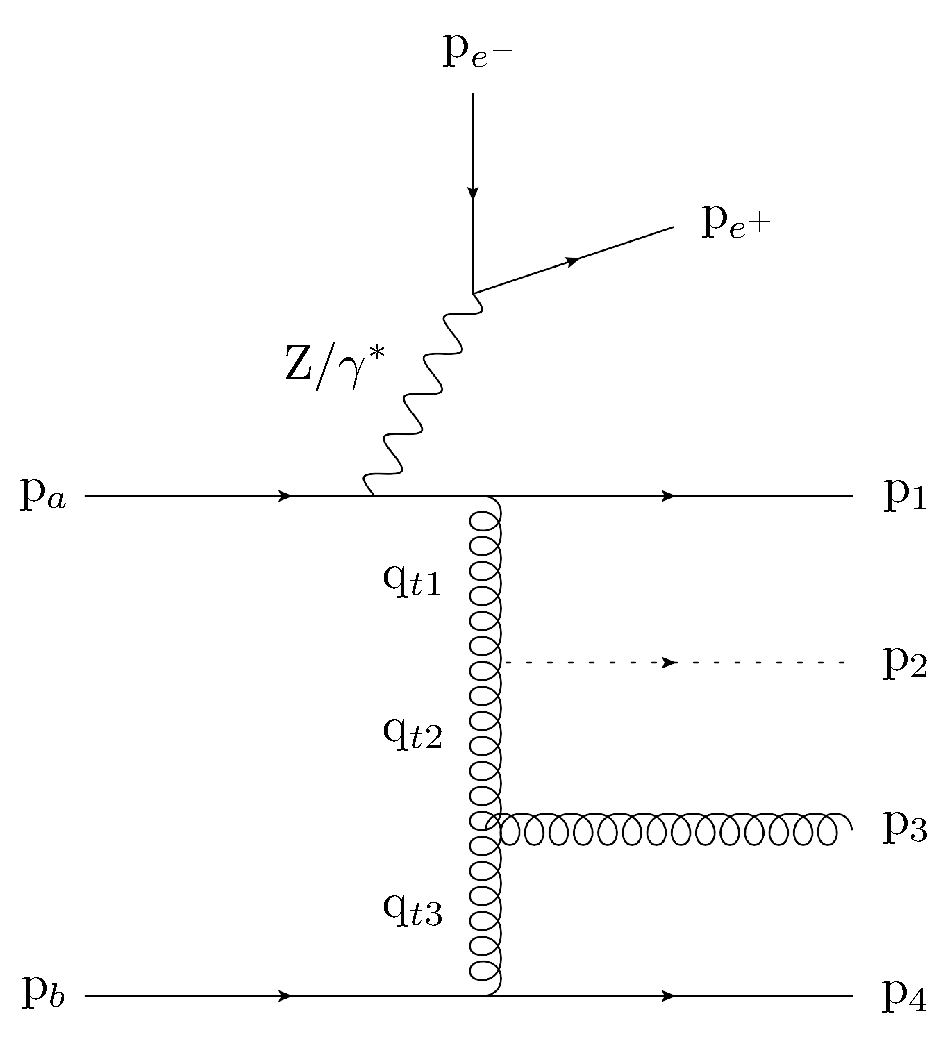
\includegraphics[width=0.5\textwidth]{figures/RealSoftEmissionZ.pdf}
			\caption{Soft Emission}
			\label{fig:real24}
		\end{subfigure}\qquad\qquad
		\begin{subfigure}[b]
			\centering
			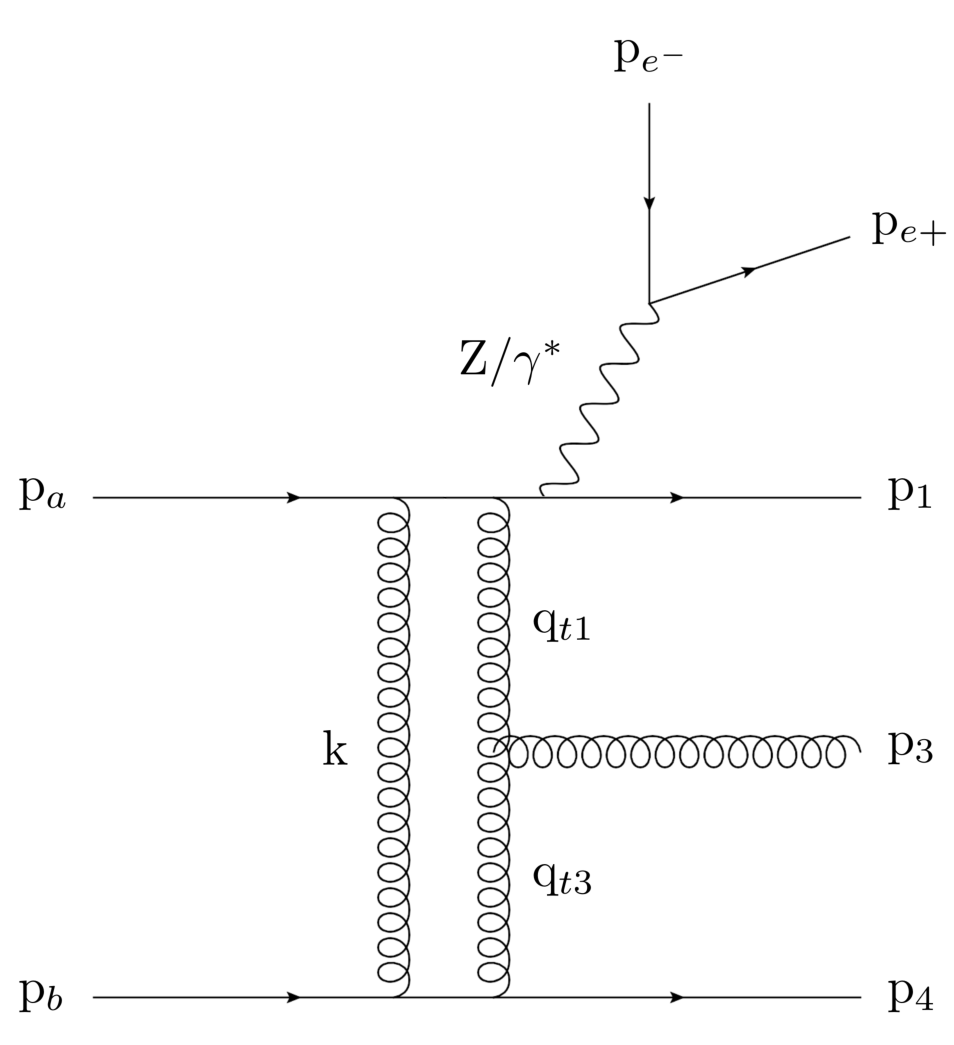
\includegraphics[width=0.5\textwidth]{figures/VirtualSoftEmissionZ.pdf}
			\caption{Virtual Emission}
			\label{fig:virtual24}
		\end{subfigure}
		\caption{Examples of diagrams contributing to $2\rightarrow4$ scattering.  In figure \ref{fig:real24} the $p_2$ has been drawn with a dashed line to denote it is not resolvable.  In figure \ref{fig:virtual24} the final state momenta have been labelled in a seemingly strange way - this was done to make clear the cancellation when working through the algebra.}
		\label{fig:2to4}
		\end{figure}

		As an example we show the cancellation explicitly for the case of $2\rightarrow4$ when the $p_2$ momentum has gone soft.  A contributing soft diagram is shown in figure \ref{fig:real24} and one example of a contributing virtual diagram of the same order is shown in figure \ref{fig:virtual24}.  When $p_2$ goes soft we have the following form for the $2\rightarrow4$ integrated amplitude squared ({N.B.}: The integration is only schematic and doesnt represent the full Lorentz invariant phase space):

		\begin{align}
		\begin{split}
		\int|\mathcal{A}^{2\rightarrow4}_{soft}|^2 = &\frac{4C_Ag_s^2\Delta_{1,3}}{(2\pi)^{2+2\epsilon}4\pi}\frac{\pi^{\epsilon+1}}{\epsilon\Gamma(\epsilon+1)}
		\left(\frac{\lambda^2}{\mu^2}\right)^\epsilon\Bigg[|\mathcal{K}_aj_1^Z\cdot j_2|^2 \frac{V^2(q_{t1}, q_{t3})}{q^2_{t1}q^2_{t3}} + |\mathcal{K}_bj_1\cdot j_2^Z|^2 \frac{V^2(q_{b1}, q_{b3})}{q^2_{b1}q^2_{b3}} + \ldots \\
		& 2\Re\left\{\mathcal{K}_a\overline{\mathcal{K}_b}  (j_1^Z\cdot j_2)\overline{(j_1\cdot j_2^Z)}\right\} \frac{V(q_{t1}, q_{t3})\cdot V(q_{b1}, q_{b3})}{q_{t1}q_{t3}q_{b1}q_{b3}}\Bigg],
		\end{split}
		\end{align}

		and the virtual contributions for the $2\rightarrow3$ amplitude is:

		\begin{align}
		\begin{split}
		\int|\mathcal{A}^{2\rightarrow3}_{virtual}|^2 = &|\mathcal{K}_bj_1\cdot j_2^Z|^2 \frac{V^2(q_{t1}, q_{t3})}{q_{t1}^2}e^{2\hat{\alpha}(q_{t1})\Delta_{1,3}} + |\mathcal{K}_tj_1^Z\cdot j_2|^2 \frac{V^2(q_{b1}, q_{b3})}{q_{b1}^2}e^{2\hat{\alpha}(q_{b1})\Delta_{1,3}} + \ldots \\
		& 2\Re\left\{\mathcal{K}_a\overline{\mathcal{K}_b}  (j_1^Z\cdot j_2)\overline{(j_1\cdot j_2^Z)}\right\} \frac{V(q_{t1}, q_{t3})\cdot V(q_{b1}, q_{b3})}{q_{t1}q_{t3}q_{b1}q_{b3}}e^{(\hat{\alpha}(q_{t1}) + \hat{\alpha}(q_{b1}))\Delta_{1,3}}.
		\end{split}
		\end{align}

		Once we expand the exponential to the correct order in $g_s^2$, the sum of these matrix elements squared over the region of phase space when $p_2$ is soft is:

		\begin{align}
		\begin{split}
		\int\left(|\mathcal{A}^{2\rightarrow4}_{soft}|^2 + |\mathcal{A}^{2\rightarrow3}_{virtual}|^2\right) = &|\mathcal{K}_aj_1^Z\cdot j_2|^2 \frac{V^2(q_{t1}, q_{t3})}{q_{t1}^2} {\Bigg(\frac{4C_Ag_s^2\Delta_{1,3}}{(2\pi)^{2+2\epsilon}4\pi}\frac{\pi^{\epsilon+1}}{\epsilon\Gamma(\epsilon+1)} - 2\hat{\alpha}(q_{t1})\Delta_{1,3}\Bigg)}+\ldots \\
		& |\mathcal{K}_bj_1\cdot j_2^Z|^2 \frac{V^2(q_{b1}, q_{b3})}{q_{b1}^2} {\Bigg(\frac{4C_Ag_s^2\Delta_{1,3}}{(2\pi)^{2+2\epsilon}4\pi}\frac{\pi^{\epsilon+1}}{\epsilon\Gamma(\epsilon+1)} - 2\hat{\alpha}(q_{b1})\Delta_{1,3}\Bigg)}+\ldots \\
		 2\Re\left\{\mathcal{K}_a\overline{\mathcal{K}_b}  (j_1^Z\cdot j_2)\overline{(j_1\cdot j_2^Z)}\right\}&\frac{V(q_{t1}, q_{t3})\cdot V(q_{b1}, q_{b3})}{q_{t1}q_{t3}q_{b1}q_{b3}}{\Bigg(\frac{4C_Ag_s^2\Delta_{1,3}}{(2\pi)^{2+2\epsilon}4\pi}\frac{\pi^{\epsilon+1}}{\epsilon\Gamma(\epsilon+1)} - (\hat{\alpha}(q_{t1}) + \hat{\alpha}(q_{b1}))\Delta_{1,3}\Bigg)} + \mathcal{O}(g_s^4),\\
		\end{split}
		\end{align}

		These bracketed terms are exactly the cancellations calculated in section 4 above.  Therefore:

		\begin{align}
		\begin{split}
		\int\left(|\mathcal{A}^{2\rightarrow4}_{soft}|^2 + |\mathcal{A}^{2\rightarrow3}_{virtual}|^2\right) = \frac{\alpha_sC_A\Delta_{1,3}}{\pi}\Bigg(&|\mathcal{K}_aj_1^Z\cdot j_2|^2 \frac{V^2(q_{t1}, q_{t3})}{q_{t1}^2}\ln\left(\frac{\lambda^2}{|q_{1t\perp}|^2}\right)+\ldots \\
		& |\mathcal{K}_bj_1\cdot j_2^Z|^2 \frac{V^2(q_{b1}, q_{b3})}{q_{b1}^2}\ln\left(\frac{\lambda^2}{|q_{1b\perp}|^2}\right)+\ldots \\
		 2\Re\left\{\mathcal{K}_a\overline{\mathcal{K}_b}  (j_1^Z\cdot j_2)\overline{(j_1\cdot j_2^Z)}\right\}&\frac{V(q_{t1}, q_{t3})\cdot V(q_{b1}, q_{b3})}{q_{t1}q_{t3}q_{b1}q_{b3}}\ln\left(\frac{\lambda^2}{\sqrt{|q_{1t\perp}|^2|q_{1b\perp}|^2}}\right)\Bigg) + \mathcal{O}(\alpha_s^2),\\
		\end{split}
		\end{align}

		Which is manifestly finite.

